\documentclass[12pt, a4paper]{book}

\usepackage[english]{babel}
\usepackage[T1]{fontenc}
\usepackage[utf8]{inputenc}
\usepackage{lmodern}
\usepackage{listings}
\usepackage{tikz}
\usepackage{amsmath}
\usepackage{amssymb}
\usepackage{framed}
\usepackage{listings}

\usetikzlibrary{arrows, chains, decorations}

\author{Florian Thuin}
\title{LSINF2224 - Programming methods}

\begin{document}
    \maketitle
    \tableofcontents
%%%%%%%%%%%%%%%%%%%%%%%%%%%%%%%%%%%%%%%%%%%%%%%%%%%%%%%%%%%%%%%%%%%%%%%%%%%%%%%%
% SECTION : Organization
%%%%%%%%%%%%%%%%%%%%%%%%%%%%%%%%%%%%%%%%%%%%%%%%%%%%%%%%%%%%%%%%%%%%%%%%%%%%%%%%
  \section{Organization}
  \label{sec:Organization}

  \subsection{Objectives}
  \label{sub:Objectives}
  \subsection{Synopsis}
  \label{sub:Synopsis}
  \subsection{Website}
  \label{sub:Website}
  \subsection{Course Outline}
  \label{sub:Course Outline}
  \subsection{Course material}
  \label{sub:Course material}
  \subsection{Bibliography}
  \label{sub:Bibliography}
  \subsection{Labs}
  \label{sub:Labs}
  \subsubsection{Goals}
  \label{subs:Goals}
  \subsubsection{Implementation}
  \label{subs:Implementation}
  \subsubsection{Languages}
  \label{subs:Languages}
  \subsubsection{Software}
  \label{subs:Software}
  \subsubsection{Assignments}
  \label{subs:Assignments}
  \subsection{Evaluation}
  \label{sub:Evaluation}


%%%%%%%%%%%%%%%%%%%%%%%%%%%%%%%%%%%%%%%%%%%%%%%%%%%%%%%%%%%%%%%%%%%%%%%%%%%%%%%%
% SECTION : Demonstration
%%%%%%%%%%%%%%%%%%%%%%%%%%%%%%%%%%%%%%%%%%%%%%%%%%%%%%%%%%%%%%%%%%%%%%%%%%%%%%%%
  \section{Demonstration}
  \label{sec:Demonstration}

  The goal of this initial demo is to show how we can automatically verify a
  Java program. We will use \textit{ESC/Java} that uses \textbf{enriched formal
  specifications} to make automated checks.

  \subsection{Binary Search: Implementation}
  \label{sub:Binary Search: Implementation}

  \lstinputlisting[language=Java, caption={Implementation of a binary search in
  Java}]{BinarySearch.java}

  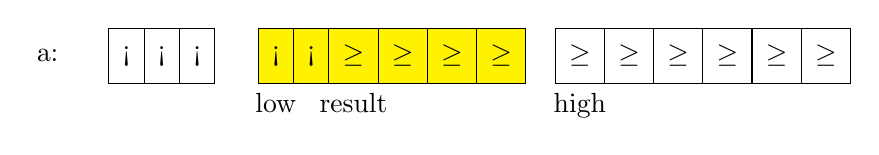
\begin{tikzpicture}
      \tikzstyle{element}=[rectangle, draw, inner sep=5pt, outer sep=0pt, minimum height=0.7cm]
      \draw (0,0) node(a) {a:};
      \node[element, right of=a] (b) {<};
      \node[element, right=0cm of b] (c) {<};
      \node[element, right=0cm of c] (d) {<};
      \node[element, right of=d, fill=yellow] (f) {<};
      \node[below=0cm of f] (low) {low};
      \node[element, right=0cm of f, fill=yellow] (g) {<};
      \node[element, right=0cm of g, fill=yellow] (h) {$\ge$};
      \node[below=0cm of h] (result) {result};
      \node[element, right=0cm of h, fill=yellow] (i) {$\ge$};
      \node[element, right=0cm of i, fill=yellow] (j) {$\ge$};
      \node[element, right=0cm of j, fill=yellow] (k) {$\ge$};
      \node[element, right of=k] (l) {$\ge$};
      \node[below=0cm of l] (high) {high};
      \node[element, right=0cm of l] (m) {$\ge$};
      \node[element, right=0cm of m] (n) {$\ge$};
      \node[element, right=0cm of n] (o) {$\ge$};
      \node[element, right=0cm of o] (p) {$\ge$};
      \node[element, right=0cm of p] (q) {$\ge$};
  \end{tikzpicture}

%%%%%%%%%%%%%%%%%%%%%%%%%%%%%%%%%%%%%%%%%%%%%%%%%%%%%%%%%%%%%%%%%%%%%%%%%%%%%%%%
%%%%%%%%%%%%%%%%%%%%%%%%%%%%%%%%%%%%%%%%%%%%%%%%%%%%%%%%%%%%%%%%%%%%%%%%%%%%%%%%
% CHAPTER : Foundations
%%%%%%%%%%%%%%%%%%%%%%%%%%%%%%%%%%%%%%%%%%%%%%%%%%%%%%%%%%%%%%%%%%%%%%%%%%%%%%%%
%%%%%%%%%%%%%%%%%%%%%%%%%%%%%%%%%%%%%%%%%%%%%%%%%%%%%%%%%%%%%%%%%%%%%%%%%%%%%%%%
  \chapter{Foundations}
  \label{chap:Foundations}

%%%%%%%%%%%%%%%%%%%%%%%%%%%%%%%%%%%%%%%%%%%%%%%%%%%%%%%%%%%%%%%%%%%%%%%%%%%%%%%%
% SECTION : Introduction
%%%%%%%%%%%%%%%%%%%%%%%%%%%%%%%%%%%%%%%%%%%%%%%%%%%%%%%%%%%%%%%%%%%%%%%%%%%%%%%%
  \section{Introduction}
  \label{sec:Introduction}
%%%%%%%%%%%%%%%%%%%%%%%%%%%%%%%%%%%%%%%%%%%%%%%%%%%%%%%%%%%%%%%%%%%%%%%%%%%%%%%%
 % SECTION : Foundations
%%%%%%%%%%%%%%%%%%%%%%%%%%%%%%%%%%%%%%%%%%%%%%%%%%%%%%%%%%%%%%%%%%%%%%%%%%%%%%%%
  \section{Foundations}
  \label{sec:Foundations}

\lstset{morekeywords={if,else,do,while}}
\begin{lstlisting}
stmt  ::= var=expr;
       |  {stmts}
       |  if (bexpr) then stmt else stmt
       |  while (bexpr) do stmt
stmts ::= stmt*
\end{lstlisting}

\begin{verbatim}
expr  ::= nexpr|bexpr|...
nexpr ::= number|var|-nexpr|nexpr+nexpr|...
bexpr ::= true|false|!bexpr|bexpr&&bexpr|...
\end{verbatim}

$nexpr \subset expr$

$bexpr \subset expr$

$(S,\sigma) \longrightarrow (S',\sigma')$

$$\frac{\phi_{1} ... \phi_{n}}{\phi}$$

$$
\frac{(S,\sigma) \longrightarrow (S', \sigma')}
{(\{S\ SS\},\sigma) \longleftarrow (\{S'\ SS\}, \sigma')}
$$

$$
\frac{}
{\ \phi \ }
$$

$$
\frac{}
{(\{ \{ \} \ SS, \sigma \}) \longrightarrow (\{ SS \}, \sigma)}
$$

$$
\frac{\phi_{1} \ldots \phi_{n}}
{\phi}
$$

\begin{eqnarray}
R^{0}   & = & \{\phi \mid \frac{}{\ \phi \ } \exists R\} \\
R^{k+1} & = & R^{k} \cup \{ \phi \mid \frac{\phi_{1} \ldots \phi_{n}}{\phi}
\in R \land \phi_{1}\ldots\phi_{n} \in R^{k} \} \\
R^{*}   & = & \bigcup_{k} R^{k}
\end{eqnarray}

$$
\vdash_{R} \phi \iff \phi \in R^{*}
$$

\paragraph{Assignment V=E;}

$$
\frac{}
{(V=E;,\sigma) \longrightarrow (\{ \}, \sigma [V := \sigma (E)] )}
$$

\paragraph{Sequence \{S SS\}}

$$
\frac{(S,\sigma) \longrightarrow (S',\sigma')}
{(\{ S\ SS \} , \sigma ) \longrightarrow (\{S'\ SS\}, \sigma')}
$$

$$
\frac{}
{(\{ \{ \} SS\}, \sigma) \longrightarrow (\{ SS \}, \sigma)}
$$

\noindent \textbf{Condition} \verb#if# $(B)$ \verb#then# $S_{1}$ \verb#else# $S_{2}$

$$
\frac{}
{(\textrm{if } (B) \textrm{ then } S_{1} \textrm{ else } S_{2}, \sigma) \longrightarrow (S_{1}, \sigma)}
\ \sigma(B)
$$

$$
\frac{}
{(\textrm{if } (B) \textrm{ then } S_{1} \textrm{ else } S_{2}, \sigma) \longrightarrow (S_{2}, \sigma)}
\ \lnot\sigma(B)
$$

\noindent \textbf{Loop} \verb#while# (B) \verb#do# S

$$
\frac{}
{(\textrm{while } (B) \textrm{ do } S, \sigma) \longrightarrow (\{ S \textrm{ while } (B) \textrm{ do } S\}, \sigma)}
\sigma(B)
$$

$$
\frac{}
{(\textrm{while } (B) \textrm{ do } S, \sigma) \longrightarrow (\{ \}, \sigma)}
\lnot\sigma(B)
$$

\paragraph{Runs, Termination, Divergence}

$(S_{0}, \sigma_{0}) \longrightarrow^{*} (S_{k}, \sigma_{k})$ iff there is a
\underline{finite} sequence

$$
(S_{0}, \sigma_{0}) \longrightarrow (S_{1}, \sigma_{1}) \longrightarrow \ldots
\longrightarrow (S_{k}, \sigma_{k})
$$

$(S, \sigma)$ terminates in $\sigma'$ iff $(S, \sigma) \longrightarrow^{*} (\{\}, \sigma')$

$(S_{0}, \sigma_{0}) \longrightarrow^{\omega}$ iff there is an \underline{infinite} sequence

$$
(S_{0}, \sigma_{0}) \longrightarrow (S_{1}, \sigma_{1}) \longrightarrow \ldots
$$

$(S,\sigma)$ diverges iff $(S,\sigma) \longrightarrow^{\omega}$

\paragraph{Semantics: Partial Correctness}

We define the semantics of a program $S$ as a function $[[S]]: \sum \rightarrow 2^{\Sigma}$ \newline

initial store $\rightarrow$ final store \newline

Partial correctness semantics:
$$
[[S]](\sigma) = \{\sigma' \mid (S,\sigma) \longrightarrow^{*} (\{\}, \sigma')\}
$$
where $[[S]](\sigma)$ is the set of possible final stores after executing $S$
from $\sigma$

\paragraph{Semantics (Set-Based Version)}

For convenience, it is useful to define $[[S]]$ on sets of initial states. \newline

For a set of stores $X \subseteq \Sigma$,
$$
[[S]](X) = \bigcup_{\sigma \in X} [[S]](\sigma)
$$

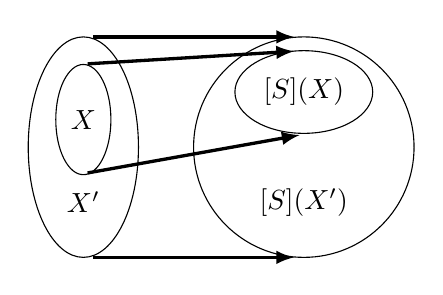
\begin{tikzpicture}[scale=0.7]
  \tikzstyle{suite}=[->,>=stealth’,thick,rounded corners=4pt]

  \draw (1,1) ellipse (1 and 2); % Right big ellipse
  \draw (1,1.5) ellipse (0.5 and 1); % Right little ellipse
  \node (A) at (1, 1.5) {$X$};
  \node (B) at (1, 0.0) {$X'$};
  \draw (5, 1) circle (2); % Right circle
  \draw (5, 2) ellipse (1.25 and 0.75); % Right ellipse in circle
  \node (C) at (5, 2) {$[S](X)$};
  \node (D) at (5, 0) {$[S](X')$};
  \node (E) at (1, 3) {}; % Top-left node
  \node (F) at (5, 3) {}; % Top-right node
  \draw[->,>=latex, very thick] (E)--(F); % Top arrow
  \node (G) at (1,-1) {};
  \node (H) at (5,-1) {};
  \draw[->,>=latex, very thick] (G)--(H); % Bottom arrow
  \node (I) at (0.9, 2.5) {};
  \node (J) at (5, 2.75) {};
  \draw[->,>=latex, very thick] (I)--(J); % Top-ellipse arrow
  \node (K) at (0.9, 0.5) {};
  \node (L) at (5.1, 1.25) {};
  \draw[->,>=latex, very thick] (K)--(L); % Bottom-ellipse arrow
\end{tikzpicture}

\paragraph{Property}: [[S]] is monotonic:

$$
X \subseteq X' \Rightarrow [[S]](X) \subseteq [[S]](X')
$$

\noindent Proof: obvious from definition \newline
Important for convergence of iterative computations \newline

\paragraph{Semantics: Total Correctness}

Distinguished value $\perp$ (bottom) denotes absence of final state (i.e.
the final state of a non-terminating program).

\textbf{Total Correctness Semantics:}
$$
{[[S]]}_{\perp}(\sigma) = [[S]](\sigma) \cup \{\perp \mid (S,\sigma) \longrightarrow^{\omega}\}
$$

${[[S]]}_{\perp}(\sigma)$ is like $[[S]](\sigma)$ plus $\perp$ if $S$ may
diverge from $\sigma$

\paragraph{Semantics: Determinism}

with the language defined so far, programs are deterministic and non-blocking.
If $S \neq \{ \}$, then there is one unique $(S',\sigma')$ such that
$(S,\sigma) \longrightarrow (S', \sigma')$. \newline

Hence $\lvert [[S]](\sigma) \rvert \le 1$ and $\lvert {[[S]]}_{\perp}(\sigma) \rvert = 1$. \\
If $S$ terminates, then $[[S]](\sigma) = {[[S]]}_{\perp}(\sigma) = \{\sigma'\}, \sigma' \neq \perp$ \\
If $S$ diverges, then $[[S]](\sigma) = \emptyset$ and ${[[S]]}_{\perp}(\sigma) = \{\perp\}$. \\
This is not true later with non-deterministic choice and concurrency.

\paragraph{Denotational Semantics}

$[[S]] : \Sigma \rightarrow 2^{\Sigma}$ is a denotation of the semantics of
program S, a mathematical object that fully describes the meaning of $S$.

\textbf{Denotational semantics} defines $[[[S]]](\sigma)$ by induction on $S$,
without resorting to the transition relation.

\begin{framed}
    \textbf{Example} : if-then-else
    $$
    [[\textrm{if } (B) \textrm{ then } S_{1} \textrm{ else } S_{2}]](X) =
    ([[S_{1}]] (X \cap [[B]])) \cup ([[S_{2}]] ( X \cap [[\lnot B]] ))
    $$
\end{framed}

In this course, we will consider operational semantics only.


%%%%%%%%%%%%%%%%%%%%%%%%%%%%%%%%%%%%%%%%%%%%%%%%%%%%%%%%%%%%%%%%%%%%%%%%%%%%%%%%
%%%%%%%%%%%%%%%%%%%%%%%%%%%%%%%%%%%%%%%%%%%%%%%%%%%%%%%%%%%%%%%%%%%%%%%%%%%%%%%%
% CHAPTER : Program proofs
%%%%%%%%%%%%%%%%%%%%%%%%%%%%%%%%%%%%%%%%%%%%%%%%%%%%%%%%%%%%%%%%%%%%%%%%%%%%%%%%
%%%%%%%%%%%%%%%%%%%%%%%%%%%%%%%%%%%%%%%%%%%%%%%%%%%%%%%%%%%%%%%%%%%%%%%%%%%%%%%%

  \chapter{Program Proofs}
  \label{chap:Program Proofs}

%%%%%%%%%%%%%%%%%%%%%%%%%%%%%%%%%%%%%%%%%%%%%%%%%%%%%%%%%%%%%%%%%%%%%%%%%%%%%%%%
% SECTION : Sequential programs
%%%%%%%%%%%%%%%%%%%%%%%%%%%%%%%%%%%%%%%%%%%%%%%%%%%%%%%%%%%%%%%%%%%%%%%%%%%%%%%%
  \section{Sequential Programs}
  \label{sec:Sequential Programs}

%%%%%%%%%%%%%%%%%%%%%%%%%%%%%%%%%%%%%%%%%%%%%%%%%%%%%%%%%%%%%%%%%%%%%%%%%%%%%%%%
% SECTION : Verification conditions
%%%%%%%%%%%%%%%%%%%%%%%%%%%%%%%%%%%%%%%%%%%%%%%%%%%%%%%%%%%%%%%%%%%%%%%%%%%%%%%%
  \section{Verification Conditions}
  \label{sec:Verification Conditions}
%%%%%%%%%%%%%%%%%%%%%%%%%%%%%%%%%%%%%%%%%%%%%%%%%%%%%%%%%%%%%%%%%%%%%%%%%%%%%%%%
% SECTION : Procedures
%%%%%%%%%%%%%%%%%%%%%%%%%%%%%%%%%%%%%%%%%%%%%%%%%%%%%%%%%%%%%%%%%%%%%%%%%%%%%%%%
  \section{Procedures}
  \label{sec:Procedures}

%%%%%%%%%%%%%%%%%%%%%%%%%%%%%%%%%%%%%%%%%%%%%%%%%%%%%%%%%%%%%%%%%%%%%%%%%%%%%%%%
% SECTION : Recursion
%%%%%%%%%%%%%%%%%%%%%%%%%%%%%%%%%%%%%%%%%%%%%%%%%%%%%%%%%%%%%%%%%%%%%%%%%%%%%%%%
  \section{Recursion}
  \label{sec:Recursion}

%%%%%%%%%%%%%%%%%%%%%%%%%%%%%%%%%%%%%%%%%%%%%%%%%%%%%%%%%%%%%%%%%%%%%%%%%%%%%%%%
% SECTION : Data Structures
%%%%%%%%%%%%%%%%%%%%%%%%%%%%%%%%%%%%%%%%%%%%%%%%%%%%%%%%%%%%%%%%%%%%%%%%%%%%%%%%
  \section{Data Structures}
  \label{sec:Data Structures}

  \section{Data abstraction}
  \label{sec:Data abstraction}


%%%%%%%%%%%%%%%%%%%%%%%%%%%%%%%%%%%%%%%%%%%%%%%%%%%%%%%%%%%%%%%%%%%%%%%%%%%%%%%%
% SECTION : Reactive Programs
%%%%%%%%%%%%%%%%%%%%%%%%%%%%%%%%%%%%%%%%%%%%%%%%%%%%%%%%%%%%%%%%%%%%%%%%%%%%%%%%
  \section{Reactive Programs}
  \label{sec:Reactive Programs}
  \subsection{From application to reactive}
  \label{sub:From application to reactive}
  \subsubsection{Applicative programs}
  \label{subs:Applicative programs}
  \subsubsection{Reactive programs}
  \label{subs:Reactive programs}
  \subsubsection{Prooofs of reactive programs}
  \label{subs:Prooofs of reactive programs}
  \subsection{Non-deterministic programs}
  \label{sub:Non-deterministic programs}
  \subsubsection{Guarded commands}
  \label{subs:Guarded commands}
  \subsubsection{Deadlock}
  \label{subs:Deadlock}
  \subsubsection{Strong vs. weak total correctness}
  \label{subs:Strong vs. weak total correctness}
  \subsection{Concurrent programs}
  \label{sub:Concurrent programs}
  \subsubsection{Interleaving}
  \label{subs:Interleaving}
  \subsubsection{Atomicity}
  \label{subs:Atomicity}
  \subsubsection{Disjoint parallel programs}
  \label{subs:Disjoint parallel programs}
  \subsubsection{Compositional proofs}
  \label{subs:Compositional proofs}
  \subsubsection{General concurrent programs}
  \label{subs:General concurrent programs}
  \subsubsection{Interference-free proofs}
  \label{subs:Interference-free proofs}
  \subsubsection{Fairness}
  \label{subs:Fairness}


%%%%%%%%%%%%%%%%%%%%%%%%%%%%%%%%%%%%%%%%%%%%%%%%%%%%%%%%%%%%%%%%%%%%%%%%%%%%%%%%
%%%%%%%%%%%%%%%%%%%%%%%%%%%%%%%%%%%%%%%%%%%%%%%%%%%%%%%%%%%%%%%%%%%%%%%%%%%%%%%%
% CHAPTER : Program validation
%%%%%%%%%%%%%%%%%%%%%%%%%%%%%%%%%%%%%%%%%%%%%%%%%%%%%%%%%%%%%%%%%%%%%%%%%%%%%%%%
%%%%%%%%%%%%%%%%%%%%%%%%%%%%%%%%%%%%%%%%%%%%%%%%%%%%%%%%%%%%%%%%%%%%%%%%%%%%%%%%

  \chapter{Program Validation}
  \label{chap:Program Validation}

%%%%%%%%%%%%%%%%%%%%%%%%%%%%%%%%%%%%%%%%%%%%%%%%%%%%%%%%%%%%%%%%%%%%%%%%%%%%%%%%
% SECTION : State-Based Models
%%%%%%%%%%%%%%%%%%%%%%%%%%%%%%%%%%%%%%%%%%%%%%%%%%%%%%%%%%%%%%%%%%%%%%%%%%%%%%%%
  \section{State-Based Models}
  \label{sec:State-Based Models}
  \subsection{Introduction}
  \label{sub:Introduction}
  \subsection{Summary}
  \label{sub:Summary}
  \subsection{Models of Reactive Programs?}
  \label{sub:Models of Reactive Programs?}
  \subsection{State machines}
  \label{sub:State machines}
  \subsubsection{Principles}
  \label{subs:Principles}
  \subsubsection{Definition}
  \label{subs:Definition}
  \subsubsection{Example}
  \label{subs:Example}
  \subsubsection{Traces}
  \label{subs:Traces}
  \subsection{Infinite executions}
  \label{sub:Infinite executions}
  \subsubsection{Example of State Machine}
  \label{subs:Example of State Machine}
  \subsection{State machines and programs}
  \label{sub:State machines and programs}
  \subsubsection{Example of Program}
  \label{subs:Example of Program}
  \subsubsection{Interpreted State Machines}
  \label{subs:Interpreted State Machines}
  \subsection{Kripke structure}
  \label{sub:Kripke structure}
  \subsubsection{Example}
  \label{subs:Example}
  \subsubsection{Interpretation on Programs}
  \label{subs:Interpretation on Programs}
  \subsection{Program Locations}
  \label{sub:Program Locations}
  \subsection{Temporal logic}
  \label{sub:Temporal logic}
  \subsection{LTL}
  \label{sub:LTL}
  \subsubsection{Principle}
  \label{subs:Principle}
  \subsubsection{Syntax}
  \label{subs:Syntax}
  \subsubsection{Semantics over traces}
  \label{subs:Semantics over traces}
  \subsubsection{Semantics over structures}
  \label{subs:Semantics over structures}
  \subsubsection{Examples (safety)}
  \label{subs:Examples (safety)}
  \subsubsection{Examples (liveness)}
  \label{subs:Examples (liveness)}
  \subsubsection{Examples (deadlock)}
  \label{subs:Examples (deadlock)}
  \subsubsection{Until vs Unless}
  \label{subs:Until vs Unless}
  \subsubsection{Quid of Hoare Logic?}
  \label{subs:Quid of Hoare Logic?}
  \subsubsection{Examples (pre/post)}
  \label{subs:Examples (pre/post)}
  \subsection{Other temporal logics}
  \label{sub:Other temporal logics}
  \subsection{Summary}
  \label{sub:Summary}






%%%%%%%%%%%%%%%%%%%%%%%%%%%%%%%%%%%%%%%%%%%%%%%%%%%%%%%%%%%
%% SECTION : MODEL CHECKING
%%%%%%%%%%%%%%%%%%%%%%%%%%%%%%%%%%%%%%%%%%%%%%%%%%%%%%%%%%%
  \section{Model Checking}
  \label{sec:Model Checking}
  \subsection{Recall}
  \label{sub:Recall}
  \subsubsection{State Machines}
  \label{subs:State Machines}
  \subsubsection{Temporal logic}
  \label{subs:Temporal logic}
  \subsubsection{Summary}
  \label{subs:Summary}
  \subsection{Definition}
  \label{sub:Definition}
  \subsection{Basic principles}
  \label{sub:Basic principles}
  \subsection{Verification vs. Refutation}
  \label{sub:Verification vs. Refutation}
  \subsection{Automata}
  \label{sub:Automata}
  \subsection{Two versions of model-checking}
  \label{sub:Two versions of model-checking}
  \subsection{Reachability}
  \label{sub:Reachability}
  \subsection{LTL property}
  \label{sub:LTL property}
  \subsection{Infinite traces}
  \label{sub:Infinite traces}
  \subsection{Büchi Automata}
  \label{sub:Büchi Automata}
  \subsubsection{From LTL to Büchi}
  \label{subs:From LTL to Büchi}
  \subsubsection{Examples}
  \label{subs:Examples}
  \subsection{Product Automaton}
  \label{sub:Product Automaton}
  \subsection{Repeated reachability}
  \label{sub:Repeated reachability}
  \subsubsection{Remarks}
  \label{subs:Remarks}
  \subsubsection{Example}
  \label{subs:Example}
  \subsubsection{Properties}
  \label{subs:Properties}
  \subsection{Model-checking without LTL?}
  \label{sub:Model-checking without LTL?}
  \subsection{Complexity}
  \label{sub:Complexity}
  \subsubsection{State space explosion}
  \label{subs:State space explosion}
  \subsection{Partial-order reduction}
  \label{sub:Partial-order reduction}
  \subsection{Spin}
  \label{sub:Spin}
  \subsubsection{Promela}
  \label{subs:Promela}
  \subsubsection{Execution}
  \label{subs:Execution}
  \subsection{Symbolic Model Checking}
  \label{sub:Symbolic Model Checking}
  \subsection{Binary Decision Diagrams (BDD)}
  \label{sub:Binary Decision Diagrams (BDD)}
  \subsubsection{Definition}
  \label{subs:Definition}
  \subsubsection{Example}
  \label{subs:Example}
  \subsubsection{Ordering of variables}
  \label{subs:Ordering of variables}
  \subsection{SAT solving}
  \label{sub:SAT solving}
  \subsection{Bounded model-checking}
  \label{sub:Bounded model-checking}
  \subsubsection{Discussion}
  \label{subs:Discussion}
  \subsection{Model Checking for Programs}
  \label{sub:Model Checking for Programs}
  \subsubsection{Traditional model checkers}
  \label{subs:Traditional model checkers}
  \subsubsection{Java PathFinder}
  \label{subs:Java PathFinder}
  \subsection{Test vs. Model checking}
  \label{sub:Test vs. Model checking}
  \subsection{Partial Model-Checking}
  \label{sub:Partial Model-Checking}
  \subsection{Exploration strategies}
  \label{sub:Exploration strategies}
  \subsection{State Hashing}
  \label{sub:State Hashing}
  \subsection{Stateless Model-Checking}
  \label{sub:Stateless Model-Checking}
  \subsubsection{Verisoft}
  \label{subs:Verisoft}
  \subsection{Runtime Monitoring}
  \label{sub:Runtime Monitoring}
  \subsection{Summary}
  \label{sub:Summary}




\end{document}
